\documentclass[]{article}

\usepackage{fancyhdr}  % Include the package for custom headers and footers

\pagestyle{fancy}  % Change the page style to fancy to apply custom headers/footers
\fancyhf{}  % Clear all header and footer fields to start fresh
\fancyhead[R]{\thepage}  % Place the page number in the top right corner of the header
\renewcommand{\headrulewidth}{0pt}  % Remove the header rule line
\usepackage{pdflscape}
\usepackage{pdfpages}
\usepackage{graphicx}
\usepackage{subcaption}
\usepackage{colortbl}
\usepackage{booktabs}
% Beamer presentation requires \usepackage{colortbl} instead of \usepackage[table,xcdraw]{xcolor}
%opening


\newenvironment{changemargin}[2]{%
	\begin{list}{}{%
			\setlength{\topsep}{0pt}%
			\setlength{\leftmargin}{#1}%
			\setlength{\rightmargin}{#2}%
			\setlength{\listparindent}{\parindent}%
			\setlength{\itemindent}{\parindent}%
			\setlength{\parsep}{\parskip}%
		}%
		\item[]}{\end{list}}
	

\title{Neural Network Classification of Top Quark Production at the Large Hadron Collider }
\author{Raveel Tejani}
\date{\parbox{\linewidth}{\centering%
		\today\endgraf\bigskip\bigskip\bigskip\bigskip\bigskip\bigskip\bigskip\bigskip\bigskip\bigskip
		\bigskip\bigskip\bigskip\bigskip\bigskip\bigskip\bigskip\bigskip\bigskip
		PHYS 310 \endgraf\bigskip
		University of British Columbia}}



\begin{document}

\maketitle
\thispagestyle{empty}
\clearpage

\tableofcontents 
\thispagestyle{empty}
\clearpage

\listoftables
\thispagestyle{empty}
\clearpage
             
\listoffigures
\thispagestyle{empty}
\clearpage     

\section{Introduction}

In high-energy physics, the Large Hadron Collider (LHC) represents the pinnacle of experimental technology, which provides insights into the fundamental particles that constitute our universe. Within the LHC, protons are accelerated to near light speeds and collided, producing a myriad of particle interactions suck as quarks that are monitored by several detectors, including the ATLAS experiment.  Top quarks are one of the six types of quarks in the Standard Model of particle physics, distinguished as the heaviest of all observed elementary particles. A top quark pair ($t\bar{t}$) consists of a top quark and its antiparticle, the top antiquark. The coupling of the top quark pair with a $Z$ boson ($t\bar{t}Z$) is particularly interesting as it is not well constrained by current data and its value can be altered by 'beyond the Standard Model' (BSM) physics processes \cite{ttZ}.

\begin{figure}[h!]
	\centering
	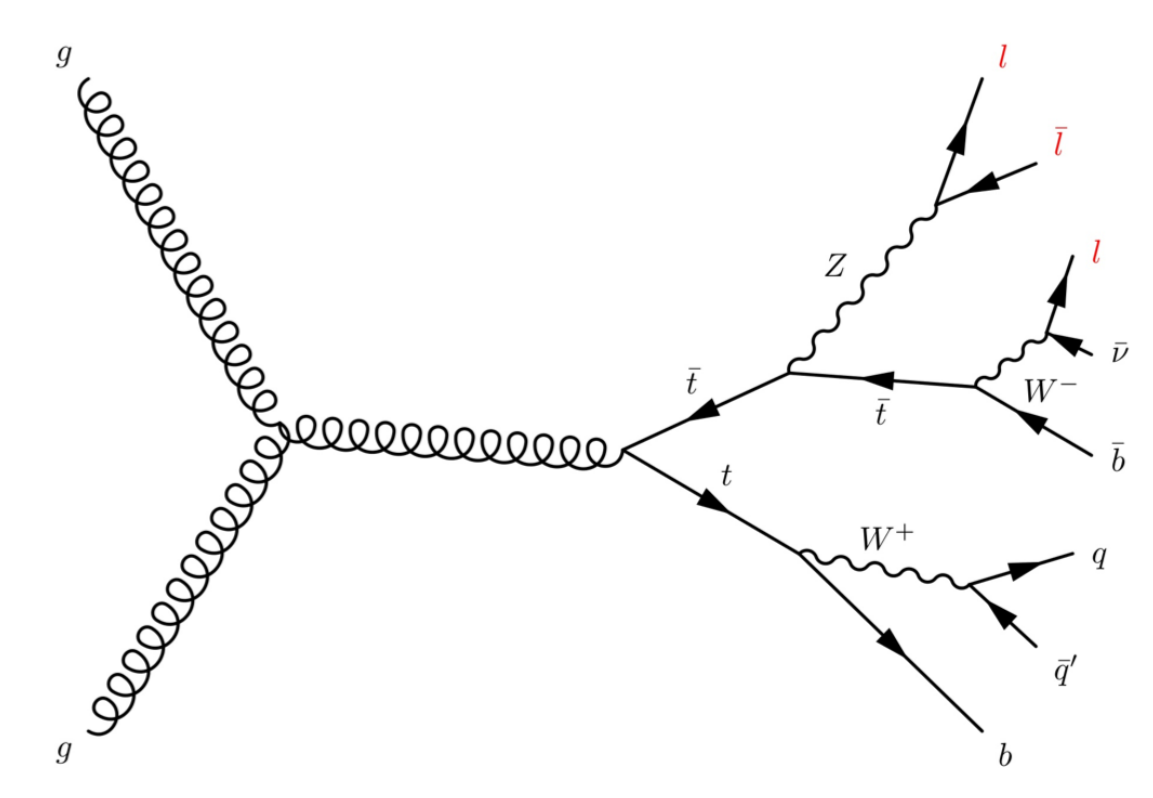
\includegraphics[width=.65\linewidth]{ttZ-feinman-diagram.png}
	\caption{A Feynman Diagram for $t\bar{t}Z$ Production \cite{ttZimage}.}
\end{figure}
The production of $t\bar{t}Z$ has the unfortunate circumstance of $W$ and $Z$ boson pairs ($WZ$) as irreducible background. Thus the challenge lies in differentiating the $t\bar{t}Z$ signal events from background events of $WZ$, which often present similar features at the detector level. Given the rarity of the $t\bar{t}Z$ events relative to these backgrounds, achieving precise separation is crucial for accurate analysis and interpretation. To this end, this study employs neural network classifiers trained on simulated data of both $t\bar{t}Z$ and $WZ$ events generated through Monte Carlo simulations. The ability of these classifiers to discern between these events based on detector-level features holds the key to isolating and studying the elusive $t\bar{t}Z$. This study not only highlights the integration of machine learning techniques in high-energy physics but also underscores the ongoing evolution of data analysis in the face of increasingly complex experimental data.




\clearpage
\section{Methods}

The initial phase of the project involved utilizing a predefined neural network (NN) model, constructed using the Sequential API within Keras, for the classification of $t\bar{t}Z$ and $WZ$ events. The base model was configured to operate with a subset of features, specifically 9 out of a possible 18 features, selected based on prior analyses which identified them as significant. 
We will perform the following steps to hopefully enhance the model's performance:

\begin{figure}[ht]

	\begin{subfigure}{\textwidth}
		\centering
		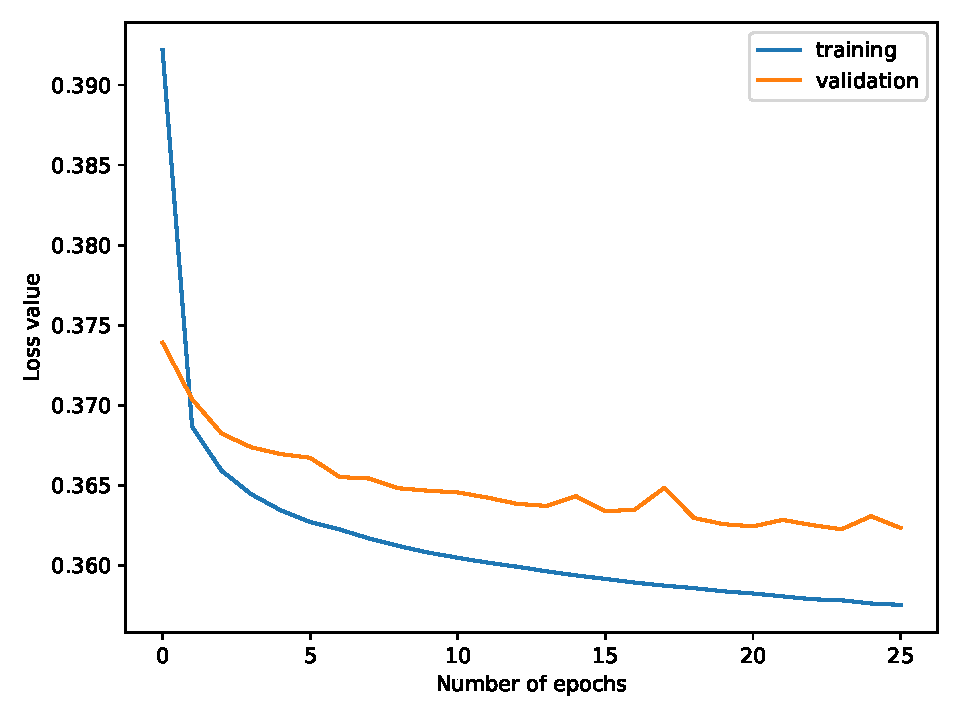
\includegraphics[height=.45\linewidth]{base_model/base_loss.pdf}
		\caption{Loss reduction as a function of epochs}
	\end{subfigure}%
	\vspace{0.2cm} % Adds space between the rows
	
	\begin{subfigure}{\textwidth}
	\centering
		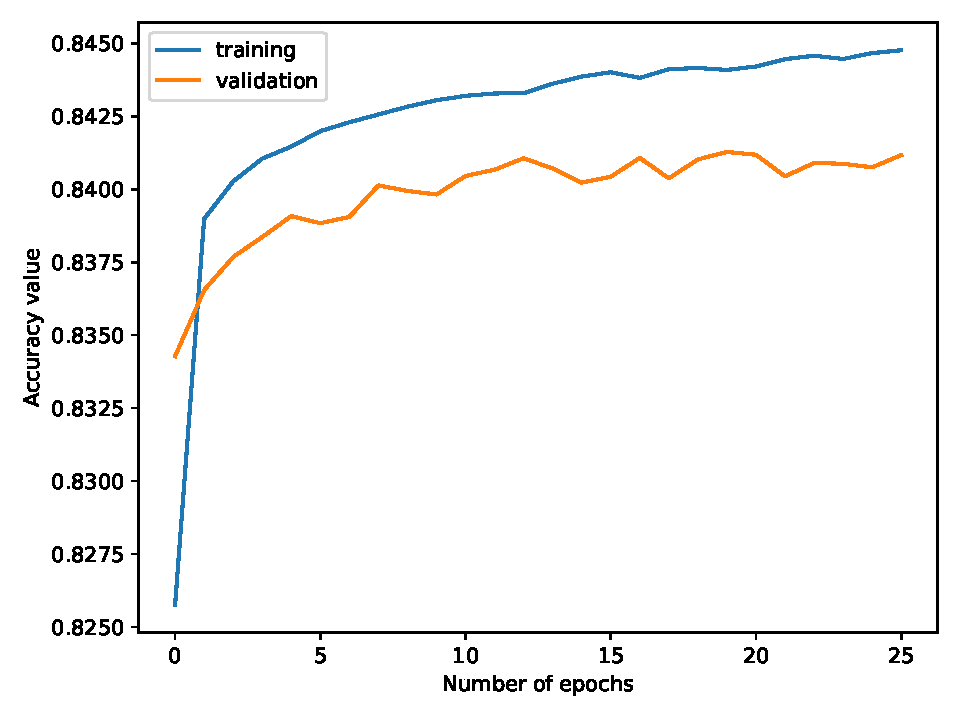
\includegraphics[height=.45\linewidth]{base_model/base_accuracy.pdf}
		\caption{Accuracy performance as a function of epochs}
	
	\end{subfigure}
	\vspace{0.2cm} % Adds space between the rows
	
	\begin{subfigure}{\textwidth}
		\centering
		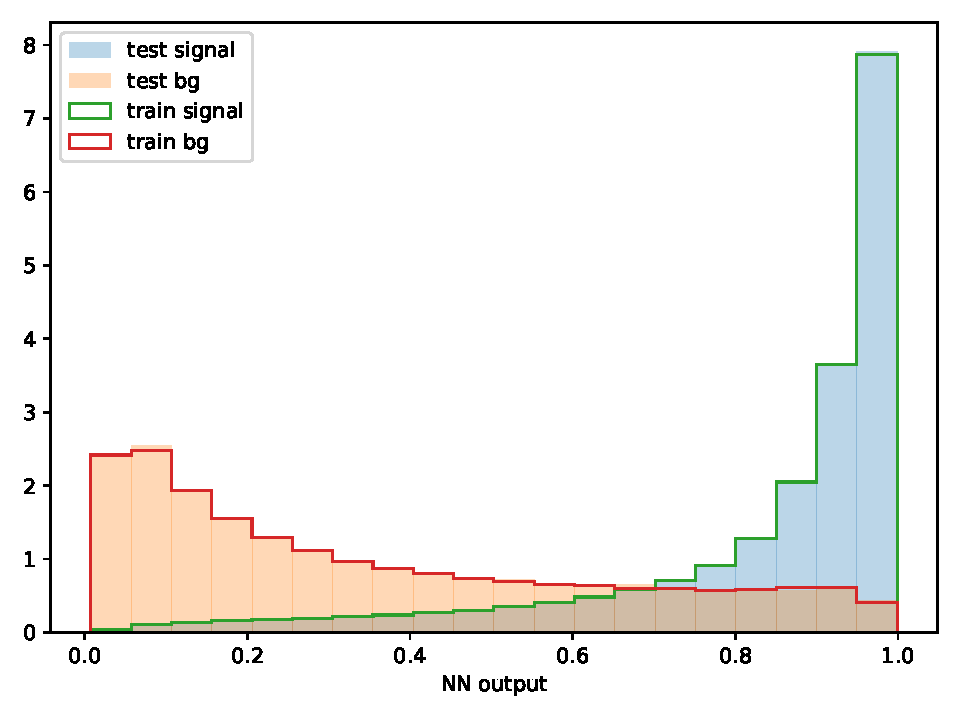
\includegraphics[height=.45\linewidth]{base_model/base_NNout.pdf}
		\caption{Probability distribution of test and train cases, based on trained Neural network}
	\end{subfigure}
	
	\caption{Performance of Base Neural Network Model Using Base Feature Selection. (a) Loss curves for the training and validation datasets, demonstrating model convergence. (b) Accuracy scores for the training and validation datasets, reflecting model effectiveness. (c) NN output distributions for both training and testing datasets, highlighting the model's differentiation between signal and background classes. Relevant code found in Appendix \ref{code_base}.}
	\label{fig:base_model_plots}
\end{figure}


\begin{enumerate}
\item \textbf{Feature Selection:}
 Sequential Feature Selector (SFS) was employed to methodically identify the most impactful features. This process resulted in two new feature sets: the "best" feature list comprising 11 of the 18 total features, and a "small" feature list which achieved comparable accuracy with only 7 out of 18 features. These subsets were chosen based on their ability to optimize the predictive accuracy of the models while minimizing complexity. Subsequent to feature selection, a comparative analysis was conducted using the base model structure with the three different sets of features: the original base feature list, the newly identified best feature list, and the small feature list. This comparison was aimed at determining the impact of each feature set on model performance in terms of accuracy.

\item \textbf{Parameter Optimization via GridSearchCV:}
Following the feature comparison, GridSearchCV was implemented to systematically explore and optimize several hyperparameters for each model variant (base, best feature list, and small feature list). The effectiveness of each model was assessed based on classification accuracy. Subsequent to GridSearchCV, a comparative analysis was conducted using the unique optimal model structure for the three different sets of features: the original base feature list, the newly identified best feature list, and the small feature list.

\item \textbf{Feature Importance Analysis:}
Finally, to understand the contribution of individual features within the optimized models, a permutation feature importance analysis was performed. This method involved systematically altering the values of each feature in the dataset and observing the resultant impact on model performance. This analysis helped to highlight which features were most critical to the model’s predictive capabilities, providing insights into the underlying data structure and the physics phenomena being modeled.
\end{enumerate}



\clearpage
\section{Results}


\subsection{Feature Selection}


We present our findings from applying Sequential Feature Selection (SFS) to our dataset. SFS, while powerful, is notably computationally intensive as it involves multiple iterations over the feature list. The process begins with a model devoid of any features, progressively incorporating features based on their contribution to performance enhancement. Given our dataset includes 18 features, this amounts to 171 evaluations:

$$18 + 17 + ....  + 1 = \frac{18 \times 19}{2} = 171 $$

Additionally, we employ cross-validation during each evaluation to enhance the robustness of our findings, leading to a total of 
$171 \times 5 =855$ model fits. Our dataset contains over $700,000$ instances. To manage the computational demands, we selectively use smaller data subsets—10,000 and 30,000 samples—and execute SFS on these subsets. The implementation details can be found in Appendix \ref{code_feat_selection}. 

The outcomes, are summarized in Figure \ref{fig:SFS_results} and Table \ref{table:SFS_results}. This approach not only aids us by identifying high performing features but also helps in optimizing processing time.  Table \ref{table:SFS_results} outlines the features selected during each iteration and their corresponding average CV accuracy, illustrating how each feature contributes to the overall model performance. Data compiled in Table \ref{table:SFS_results} is directly related to plot (b) in Figure \ref{fig:SFS_results}, providing a detailed view of the feature selection impact within this specific subset.

We have opted to advance with three distinct feature lists for our analysis. The first list is the initially suggested base list, the second is the best-performing list as determined by the SFS, and the third, also suggested by SFS, is the smallest list that maintains at least 80\% accuracy. The latter two lists are highlighted in green in Table \ref{table:SFS_results}. Utilizing the full dataset, we produced plots similar to those in Figure \ref{fig:base_model_plots} using the base NN architecure provided, and our findings are showcased in Figure \ref{fig:base_models}. The relevant code is documented in Appendix \ref{code_feat_comparison}.


	\begin{figure}[ht]
		\centering
		\begin{subfigure}{\textwidth}
			\centering
		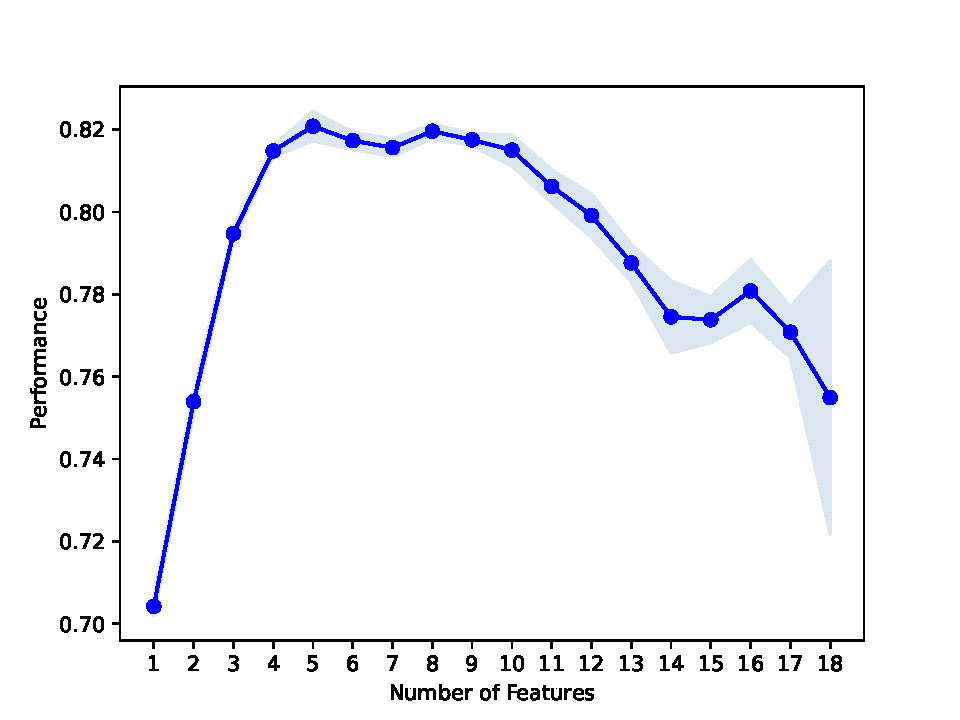
\includegraphics[width=0.9\linewidth]{feature selection/feature_num_performance_10k.pdf}
		\caption{10 000 samples}
		\end{subfigure}
		
		\begin{subfigure}{\textwidth}
		\centering
		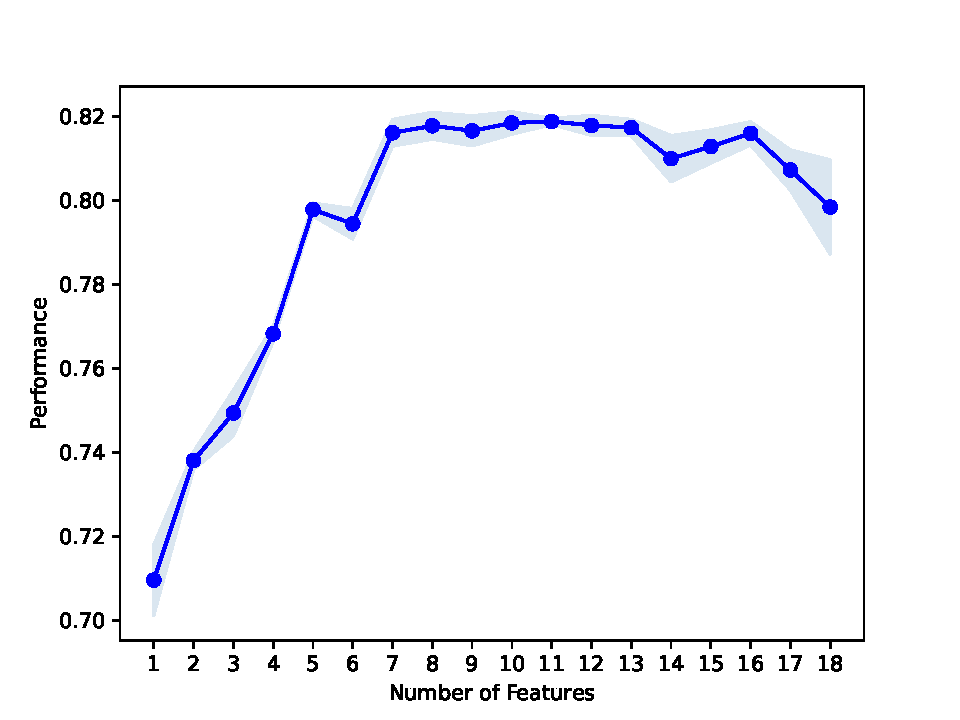
\includegraphics[width=0.9\linewidth]{feature selection/feature_num_performance_30k.pdf}
		\caption{30 000 samples}
		\end{subfigure}
		\caption{Accuracy Performance of the Sequential Feature Selector on Two Data Subsets.}
		\label{fig:SFS_results}
	\end{figure}
	
	
\begin{landscape}
\begin{table}[]
	\centering
	\resizebox{0.8\columnwidth}{!}{%
	\begin{tabular}{@{}lr@{}}
		\toprule
		Average CV Score               & Feature Names                                                                                                                                                                                                                                                                                        \\ \midrule
		70.96\%                        & ('bjet\_1\_pt',)                                                                                                                                                                                                                                                                                     \\ \addlinespace[0.5em]
		73.81\%                        & ('bjet\_1\_pt', 'n\_jets')                                                                                                                                                                                                                                                                           \\ \addlinespace[0.5em]
		74.94\%                        & ('bjet\_1\_pt', 'n\_jets', 'n\_bjets')                                                                                                                                                                                                                                                               \\ \addlinespace[0.5em]
		76.82\%                        & ('jet\_1\_twb', 'bjet\_1\_pt', 'n\_jets', 'n\_bjets')                                                                                                                                                                                                                                                \\ \addlinespace[0.5em]
		79.78\%                        & ('jet\_1\_twb', 'jet\_2\_twb', 'bjet\_1\_pt', 'n\_jets', 'n\_bjets')                                                                                                                                                                                                                                 \\ \addlinespace[0.5em]
		79.44\%                        & ('jet\_3\_pt', 'jet\_1\_twb', 'jet\_2\_twb', 'bjet\_1\_pt', 'n\_jets', 'n\_bjets')                                                                                                                                                                                                                   \\ \addlinespace[0.5em]
		\rowcolor[HTML]{32CB00} 
		81.61\%                        & ('jet\_3\_pt', 'jet\_1\_twb', 'jet\_2\_twb', 'jet\_3\_twb', 'bjet\_1\_pt',   'n\_jets', 'n\_bjets')                                                                                                                                                                                                  \\ \addlinespace[0.5em]
		81.77\%                        & \begin{tabular}[c]{@{}l@{}}('jet\_3\_pt', 'jet\_3\_eta', 'jet\_1\_twb', 'jet\_2\_twb', 'jet\_3\_twb',   'bjet\_1\_pt', 'n\_jets',\\ 'n\_bjets')\end{tabular}                                                                                                                                         \\ \addlinespace[0.5em]
		81.65\%                        & \begin{tabular}[c]{@{}l@{}}('jet\_3\_pt', 'jet\_1\_eta', 'jet\_3\_eta', 'jet\_1\_twb', 'jet\_2\_twb',   'jet\_3\_twb', 'bjet\_1\_pt',\\ 'n\_jets', 'n\_bjets')\end{tabular}                                                                                                                          \\ \addlinespace[0.5em]
		81.84\%                        & \begin{tabular}[c]{@{}l@{}}('jet\_3\_pt', 'jet\_1\_eta', 'jet\_3\_eta', 'jet\_1\_twb', 'jet\_2\_twb',   'jet\_3\_twb', 'bjet\_1\_pt',\\ 'n\_jets', 'n\_bjets', 'n\_leptons')\end{tabular}                                                                                                            \\ \addlinespace[0.5em]
		\rowcolor[HTML]{32CB00} 
		{\color[HTML]{000000} 81.88\%} & {\color[HTML]{000000} \begin{tabular}[c]{@{}l@{}}('jet\_1\_pt', 'jet\_3\_pt', 'jet\_1\_eta', 'jet\_3\_eta', 'jet\_1\_twb',   'jet\_2\_twb', 'jet\_3\_twb',\\ 'bjet\_1\_pt', 'n\_jets', 'n\_bjets', 'n\_leptons')\end{tabular}}                                                                       \\ \addlinespace[0.5em]
		81.78\%                        & \begin{tabular}[c]{@{}l@{}}('jet\_1\_pt', 'jet\_3\_pt', 'jet\_1\_eta', 'jet\_3\_eta', 'jet\_1\_twb',   'jet\_2\_twb', 'jet\_3\_twb',\\ 'bjet\_1\_pt', 'lep\_1\_pt', 'n\_jets', 'n\_bjets',   'n\_leptons')\end{tabular}                                                                              \\ \addlinespace[0.5em]
		81.73\%                        & \begin{tabular}[c]{@{}l@{}}('jet\_1\_pt', 'jet\_3\_pt', 'jet\_1\_eta', 'jet\_2\_eta', 'jet\_3\_eta',   'jet\_1\_twb', 'jet\_2\_twb',\\ 'jet\_3\_twb', 'bjet\_1\_pt', 'lep\_1\_pt', 'n\_jets',   'n\_bjets', 'n\_leptons')\end{tabular}                                                               \\ \addlinespace[0.5em]
		80.99\%                        & \begin{tabular}[c]{@{}l@{}}('jet\_1\_pt', 'jet\_3\_pt', 'jet\_1\_eta', 'jet\_2\_eta', 'jet\_3\_eta',   'jet\_1\_twb', 'jet\_2\_twb',\\ 'jet\_3\_twb', 'bjet\_1\_pt', 'lep\_1\_pt', 'n\_jets',   'n\_bjets', 'n\_leptons', 'H\_T')\end{tabular}                                                       \\ \addlinespace[0.5em] 
		81.28\%                        & \begin{tabular}[c]{@{}l@{}}('jet\_1\_pt', 'jet\_3\_pt', 'jet\_1\_eta', 'jet\_2\_eta', 'jet\_3\_eta',   'jet\_1\_twb', 'jet\_2\_twb',\\ 'jet\_3\_twb', 'bjet\_1\_pt', 'lep\_1\_pt', 'n\_jets',   'n\_bjets', 'n\_leptons', 'met\_met', 'H\_T')\end{tabular}                                           \\ \addlinespace[0.5em]
		81.59\%                        & \begin{tabular}[c]{@{}l@{}}('jet\_1\_pt', 'jet\_3\_pt', 'jet\_1\_eta', 'jet\_2\_eta', 'jet\_3\_eta',   'jet\_1\_twb', 'jet\_2\_twb',\\ 'jet\_3\_twb', 'bjet\_1\_pt', 'lep\_1\_pt', 'lep\_2\_pt',   'n\_jets', 'n\_bjets', 'n\_leptons', 'met\_met', 'H\_T')\end{tabular}                             \\ \addlinespace[0.5em]
		80.72\%                        & \begin{tabular}[c]{@{}l@{}}('jet\_1\_pt', 'jet\_3\_pt', 'jet\_1\_eta', 'jet\_2\_eta', 'jet\_3\_eta',   'jet\_1\_twb', 'jet\_2\_twb',\\ 'jet\_3\_twb', 'bjet\_1\_pt', 'lep\_1\_pt', 'lep\_2\_pt',   'lep\_3\_pt', 'n\_jets', 'n\_bjets', 'n\_leptons', 'met\_met', 'H\_T')\end{tabular}               \\ \addlinespace[0.5em]
		79.84\%                        & \begin{tabular}[c]{@{}l@{}}('jet\_1\_pt', 'jet\_2\_pt', 'jet\_3\_pt', 'jet\_1\_eta', 'jet\_2\_eta',   'jet\_3\_eta', 'jet\_1\_twb', 'jet\_2\_twb',\\ 'jet\_3\_twb', 'bjet\_1\_pt', 'lep\_1\_pt',   'lep\_2\_pt', 'lep\_3\_pt', 'n\_jets', 'n\_bjets', 'n\_leptons', 'met\_met', 'H\_T')\end{tabular} \\ \bottomrule
	\end{tabular}
	}
	\caption{Iterative Feature Selection and Corresponding Average Cross-Validation Accuracy Scores by Sequential Feature Selector (SFS) for the 30,000 Sample Subset. The two highlighed rows represent the best performing feature list and the smallest list with over $80\%$ accuracy.}
	\label{table:SFS_results}
\end{table}

\end{landscape}

\begin{figure}[h!]
	\centering
	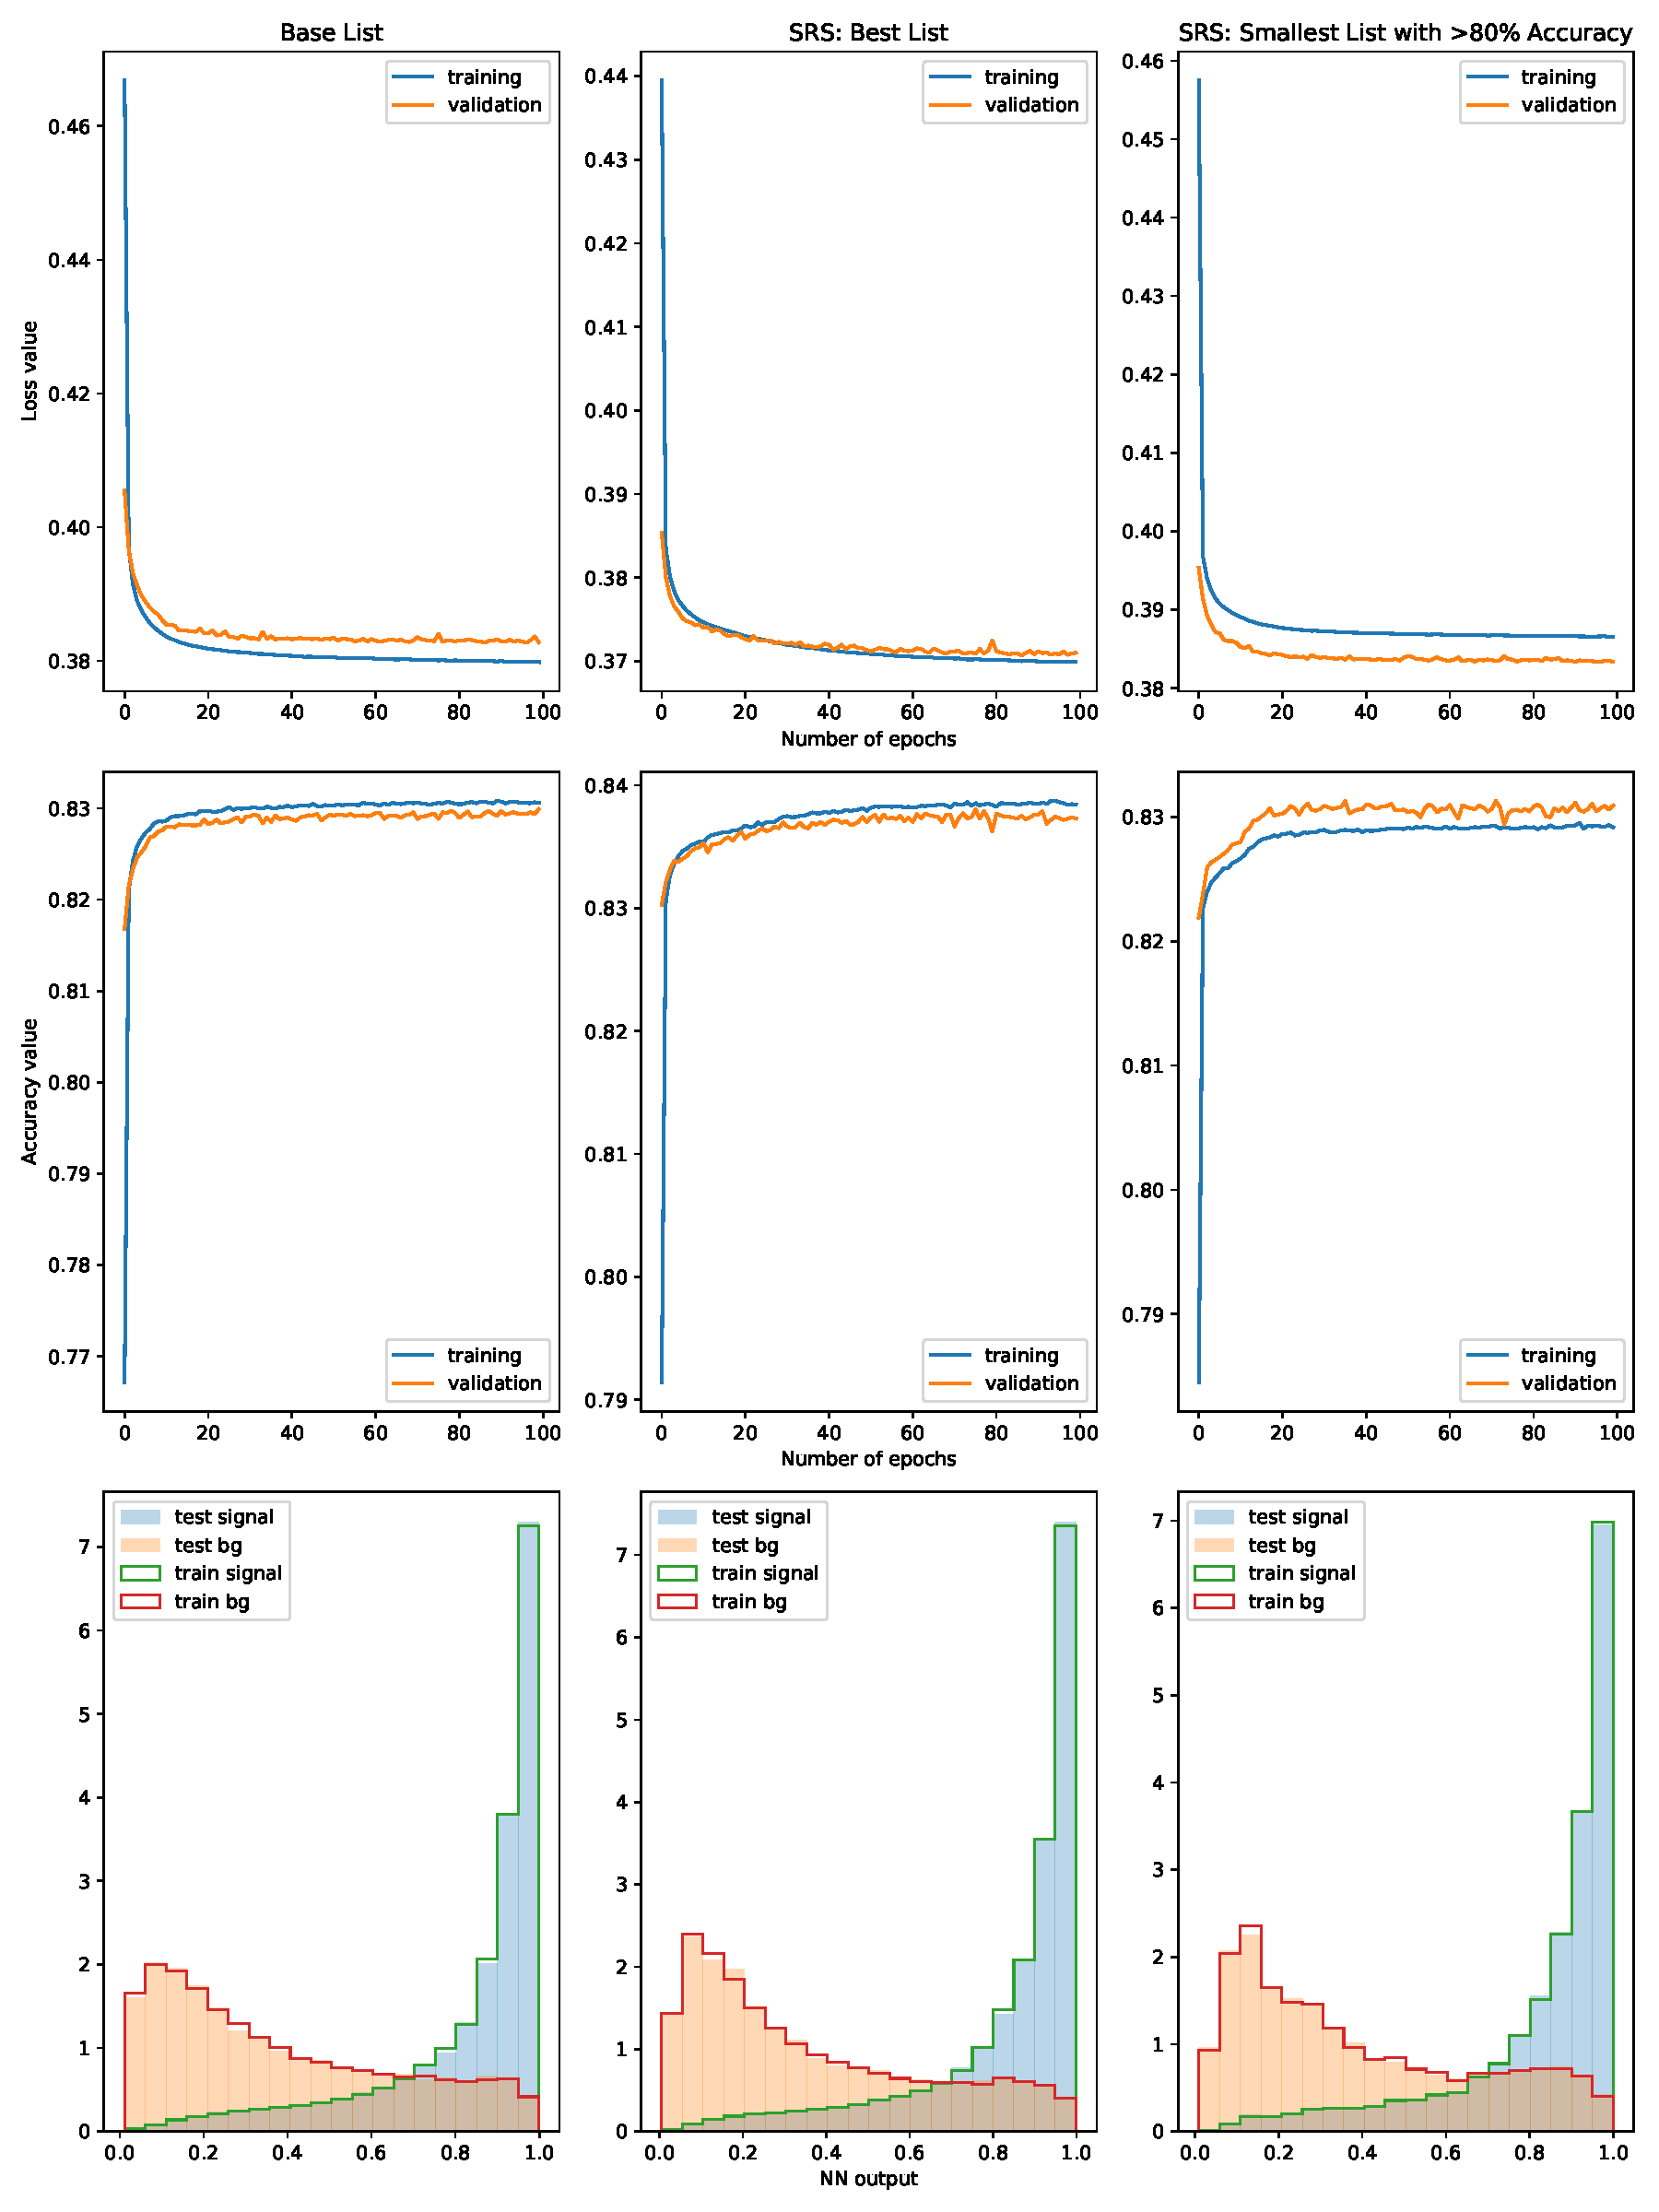
\includegraphics[width=\linewidth]{feature_comparison/feat-comparison.pdf}
	\caption{Performance Comparison of the Base Neural Network Model Using Different Feature Lists. Top panels show loss curves for the base list, SFS best list, and smallest list with over $80\%$ accuracy across training and validation phases over 100 epochs. Middle panels depict corresponding accuracy values. Bottom panels illustrate NN output distributions for training and testing datasets, highlighting model behavior for signal and background classes.}
	\label{fig:base_models}
\end{figure}

\clearpage

\subsection{Parameter Optimization via GridSearchCV}

We detail our findings from using GridSearchCV on three feature lists identified previously. The optimization adjusted parameters including the number of nodes in three neural network layers, learning rate, and batch size, with three possible values for each of these five parameters, as shown in Table \ref{table:gridsearchCV_params}. Notably, all Option 2 parameters are those used in the base model. This exhaustive search involved $3^7 = 2187$ fits due to the parameters, threefold cross-validation, and three feature sets. Because this demanded significant computational resources, we use a smaller dataset of 30,000 samples.

The results are presented in Table \ref{table:best_params_gridsearchCV}, which displays the optimal parameters and their corresponding performances. The 'Best Score' column indicates the average accuracy across the CV folds. We then applied these optimal parameters to generate the visualizations in Figure \ref{fig:best_models}, akin to those in Figure \ref{fig:base_models}. Relevant code is available in Appendices \ref{code_model_selection} and \ref{code_best_models}.

\begin{table}[h!]
	\centering
	\begin{tabular}{@{}lrrr@{}}
		\toprule
		Parameter            & Option 1  & Option 2  & Option 3  \\ \midrule
		Nodes: Dense Layer 1 & 25     & 50     & 100    \\
		Nodes: Dense Layer 2 & 12     & 25     & 50     \\
		Nodes: Dense Layer 3 & 5      & 10     & 15     \\
		Batch Size           & 100    & 150    & 300    \\
		Adam Learning Rate   & 0.002  & 0.0002 & 0.00002 \\
		\bottomrule   
	\end{tabular}
	\caption{Parameter Configurations for GridSearchCV. These list sets of values for nodes in each dense layer, batch sizes, and learning rates. Parameters under 'Option 2' corresponds to the base model.} 
	\label{table:gridsearchCV_params}
\end{table}



\begin{table}[h!]
	\centering
	\begin{tabular}{@{}lrrr@{}}
		\toprule
		Parameters           & Base List & SRS: Best List & SRS: Best Small List \\ \midrule

		Nodes: Dense Layer 1 & 50        & 25             & 50                                                  \\
		Nodes: Dense Layer 2 & 12        & 25             & 50                                                  \\
		Nodes: Dense Layer 3 & 10        & 15             & 5                                                   \\
				Batch Size          & 300       & 100            & 150                                                 \\
		Adam Learning Rate   & 0.002     & 0.002          & 0.0002                                              \\
		Best Score           & 82.96\%   & 83.39\%        & 82.7\%  \\
		\bottomrule                                            
	\end{tabular}
	\caption{Optimized Parameter Sets and Corresponding Performance Scores from GridSearchCV for our Three Feature Lists.} 
	\label{table:best_params_gridsearchCV}
	
\end{table}




\begin{figure}[h!]
	\centering
	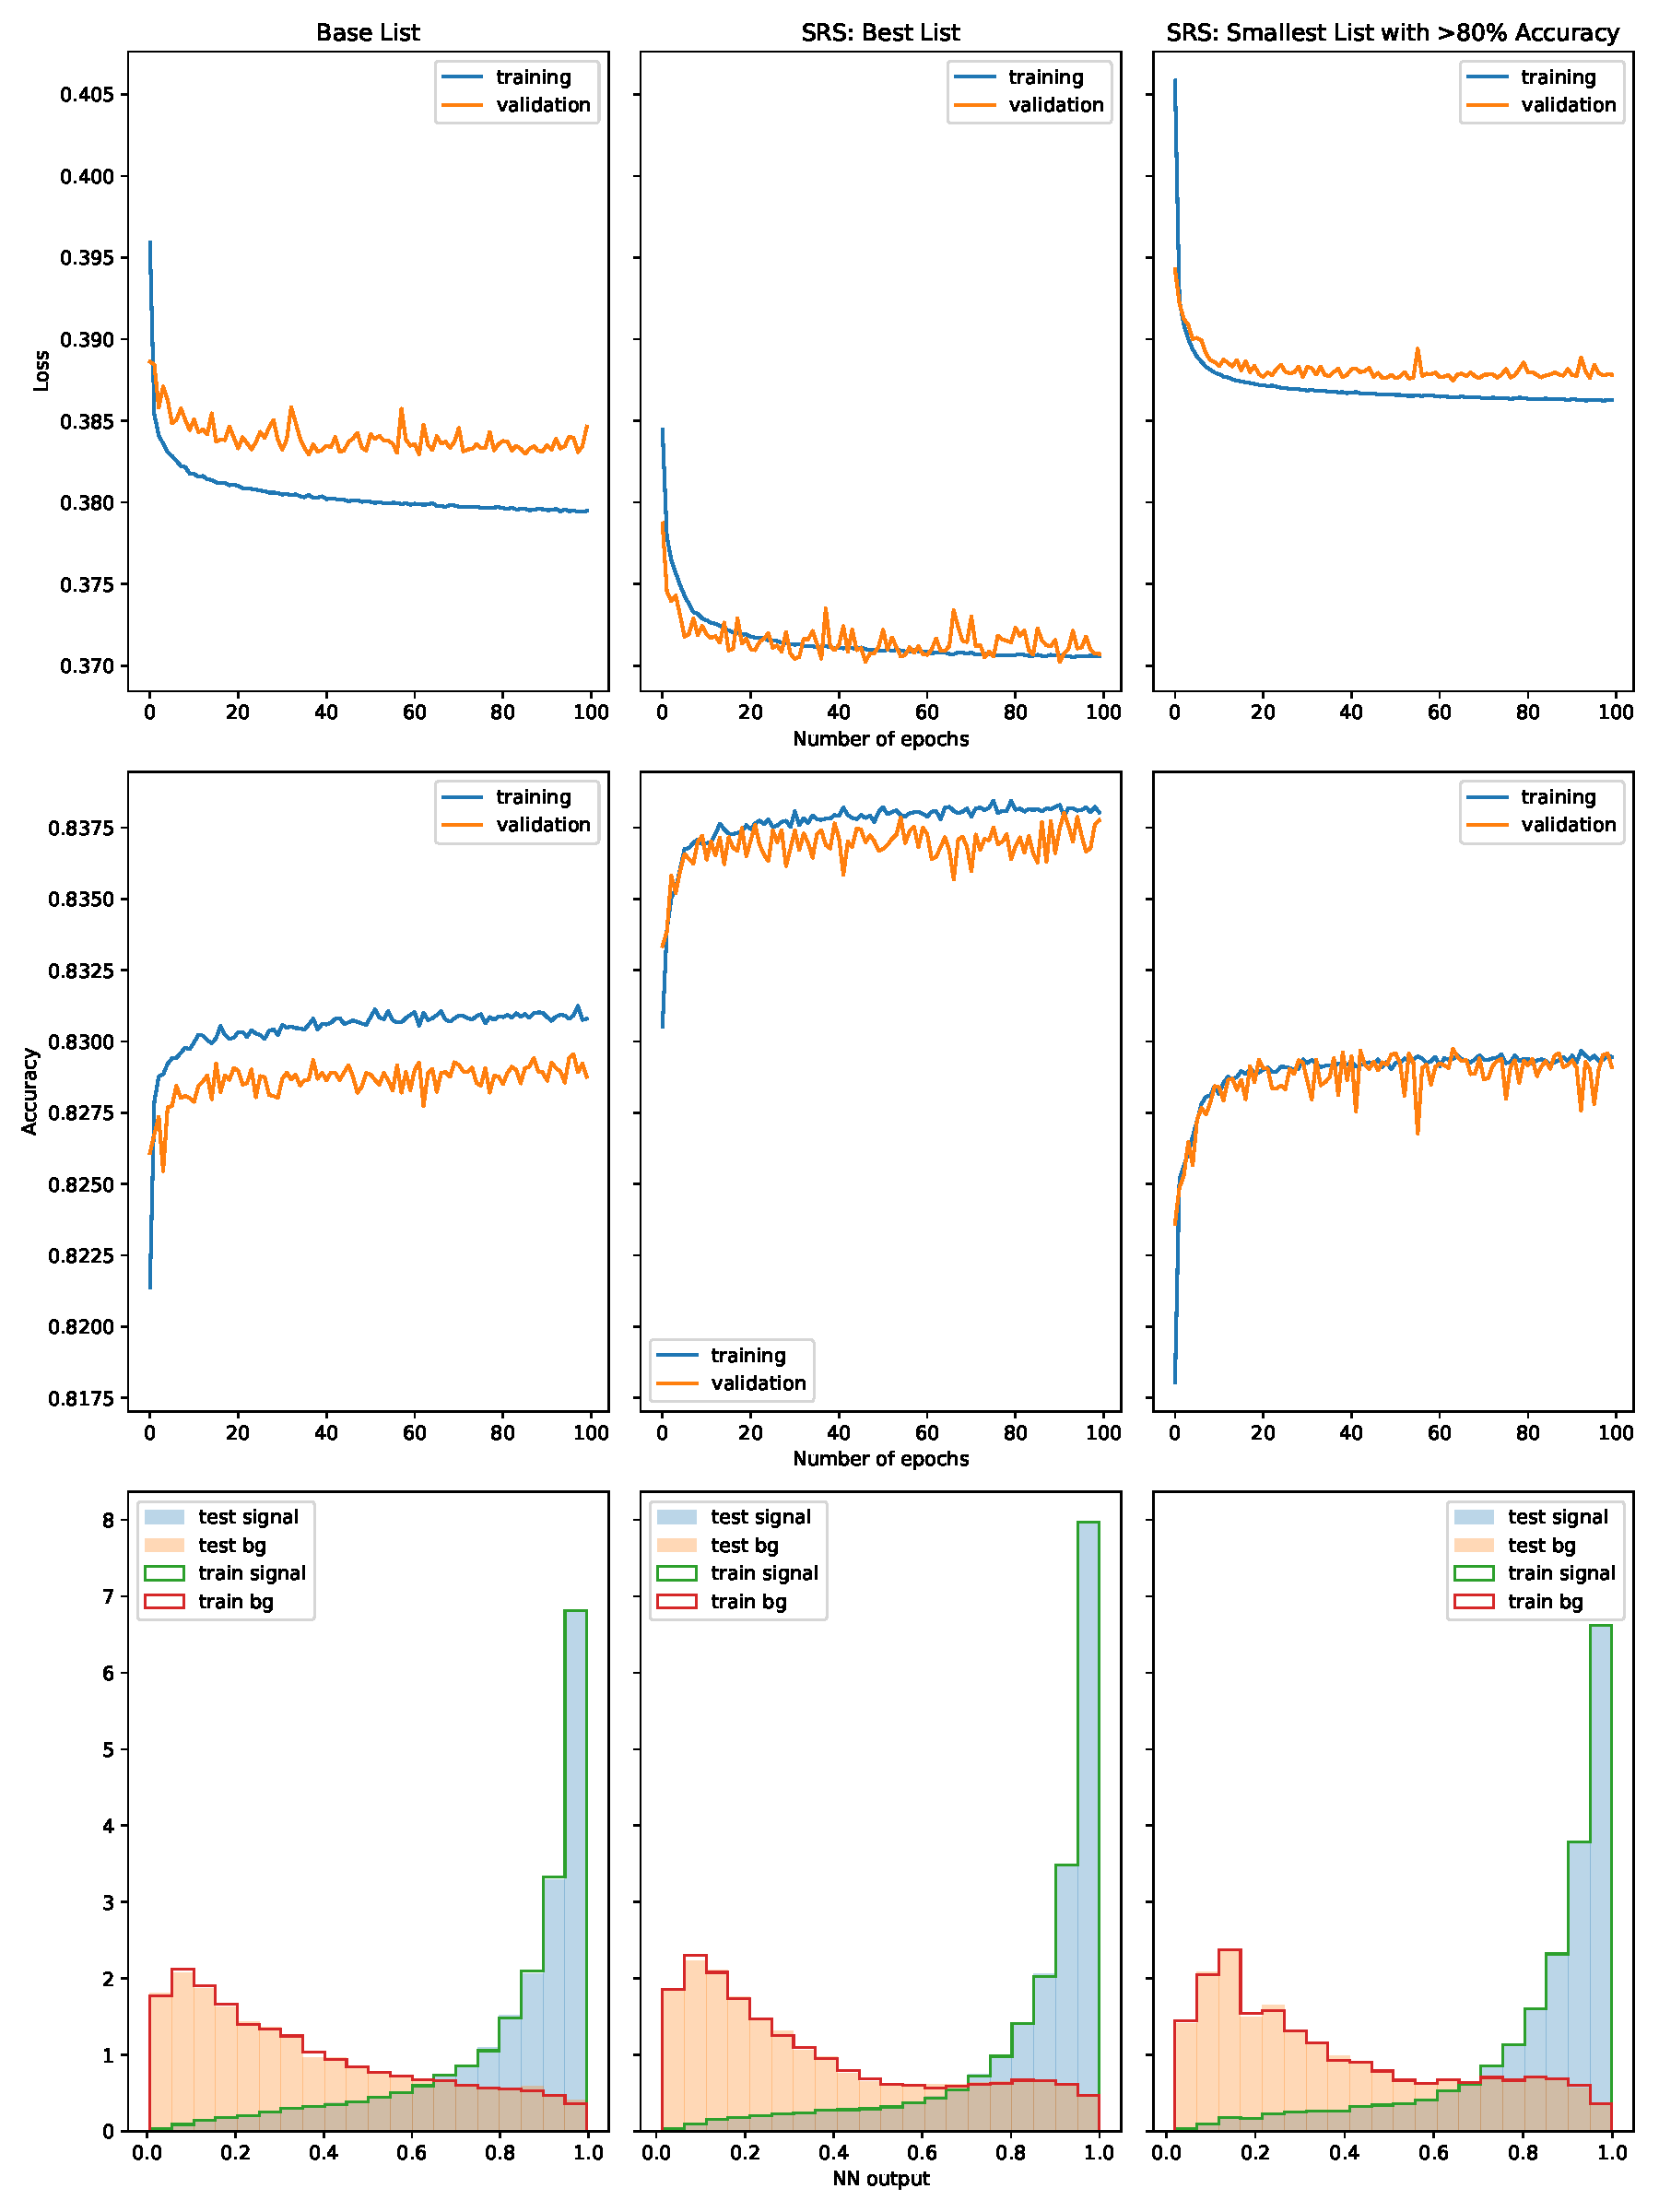
\includegraphics[width=\linewidth]{best_model/best_models.pdf}
	\caption{Performance Comparison of the Optimized Neural Network Models Using Different Feature Lists. This figure displays the outcomes of models individually optimized using GridSearchCV for the base list, the SFS best list, and the smallest list with over 80\% accuracy. Top panels show loss curves across training and validation phases over 100 epochs. Middle panels depict corresponding accuracy values. Bottom panels illustrate NN output distributions for training and testing datasets, highlighting model behavior for signal and background classes.}
	\label{fig:best_models}
\end{figure}

\clearpage

\subsection{Feature Importance Analysis}

We present our findings from conducting permutation feature importance analysis on the optimal models developed in the previous subsection. Permutation feature importance evaluates the impact of each feature on the model's performance by randomly shuffling individual feature values and observing the change in model accuracy. This process disrupts the relationship between the feature and the outcome, quantifying the importance of each feature based on the decrease in model performance. Our findings are summarized in Figure \ref{fig:best_models_feature_ranking}. This figure displays the relative importance of features across all three feature lists, highlighting how each feature contributes to model performance when utilizing the best parameters identified for each list.  The relevant code is documented in Appendix \ref{code_best_models}.

\begin{figure}[h!]
	\centering
	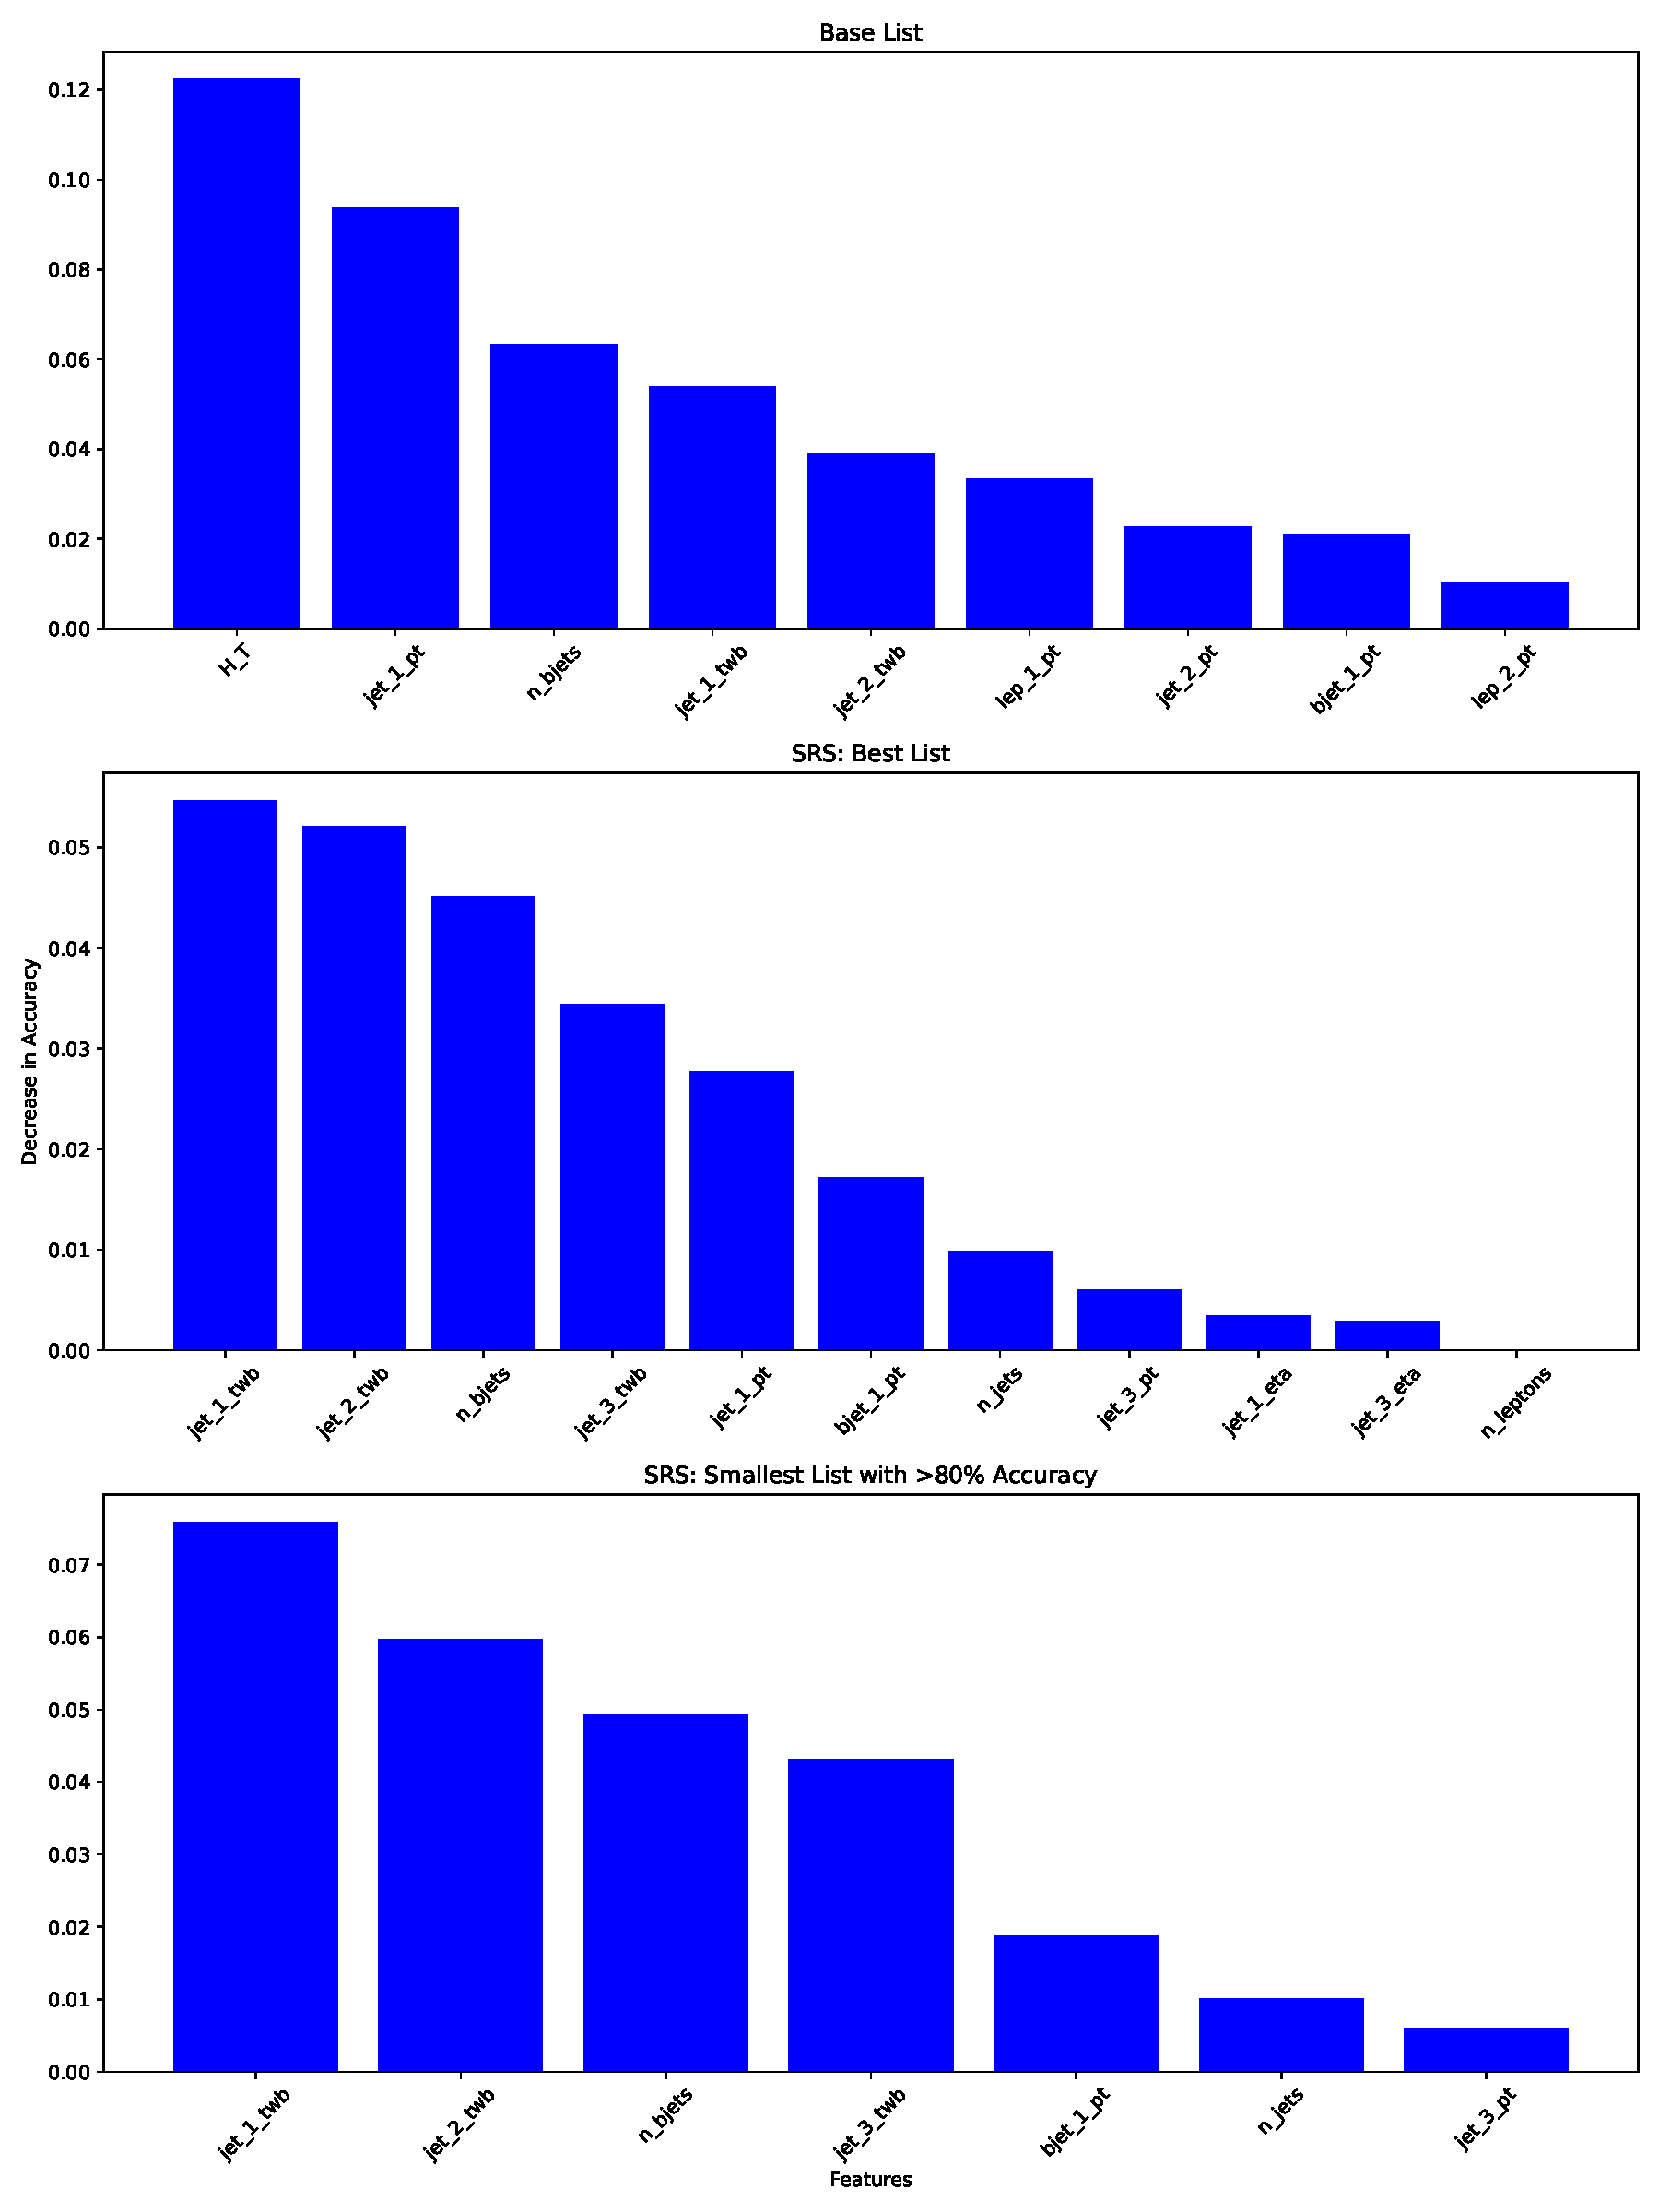
\includegraphics[width=\linewidth]{best_model/feature_importances.pdf}
	\caption{Permutation Feature Importances for Each Feature List Based on Optimized Model Parameters. }
	\label{fig:best_models_feature_ranking}
\end{figure}



\clearpage
\section{Discussion and Summary}

We did not achieve a significant improvement in accuracy in any case. Our results for each feature list, with or without the optimized parameters, resulted in accuracy hovering around $83\%$. We can see this summarized in Figures \ref{fig:base_models} and \ref{fig:best_models}.  Although SFS did not fail (provided results comparable to the base model), it also did not furnish a significant enhancement in performance. The grid search over various parameters similarly did not yield a substantial increase in accuracy.

An upside is we demonstrated the ability to reduce the dimensionality of our feature space without compromising accuracy. Our smallest feature list comprising of only 7 features performed comparably to the base list of 9 features and the optimal list of 11 features identified by SFS. Referring back to Figure \ref{fig:SFS_results}, it is evident that reducing the dimensionality to just 5 features could still preserve an accuracy close to $80\%$ and warrants further exploration.

An interesting observation emerged from the feature importance analysis. Contrary to expectations, the ranking of features in the small list from SFS did not align perfectly with those in the best list derived from SFS. For example, the feature \texttt{jet\_1\_pt} was ranked higher in the best list's feature importance despite not being in the top 7 of the SFS selections, implying it is entirely missing from the small list. Additionally, the base model identified \texttt{H\_T} as the most crucial feature, a finding SFS did not recognize until the 14th iteration, as shown in Table \ref{table:SFS_results}. This discrepancy suggests that the forward iteration approach of SFS may not have been optimal, and exploring alternative methods such as backward elimination could potentially yield different insights into feature significance.

This study underscores the complexity of feature selection and the potential limitations of certain algorithms in capturing the most predictive features. Future work could explore more dynamic feature selection methods or hybrid approaches that combine forward and backward elimination to potentially uncover more effective feature combinations. Additionally, experimenting with different model architectures or more advanced machine learning algorithms might also lead to improvements in performance. Overall, our findings suggest a continued exploration into more aspects of feature selection and model optimization to better understand classification of $t\bar{t}Z$ and $WZ$ events.

\clearpage
\bibliographystyle{unsrt}

\bibliography{references}
\addcontentsline{toc}{section}{5\;\;\;References}

\clearpage
\appendix

\clearpage
\section{Code: Base Model}\label{code_base}

We provide the code used to implement the base model introduced at the beginning of this project. This code was used in generating the visualizations displayed in Figure \ref{fig:base_model_plots}.

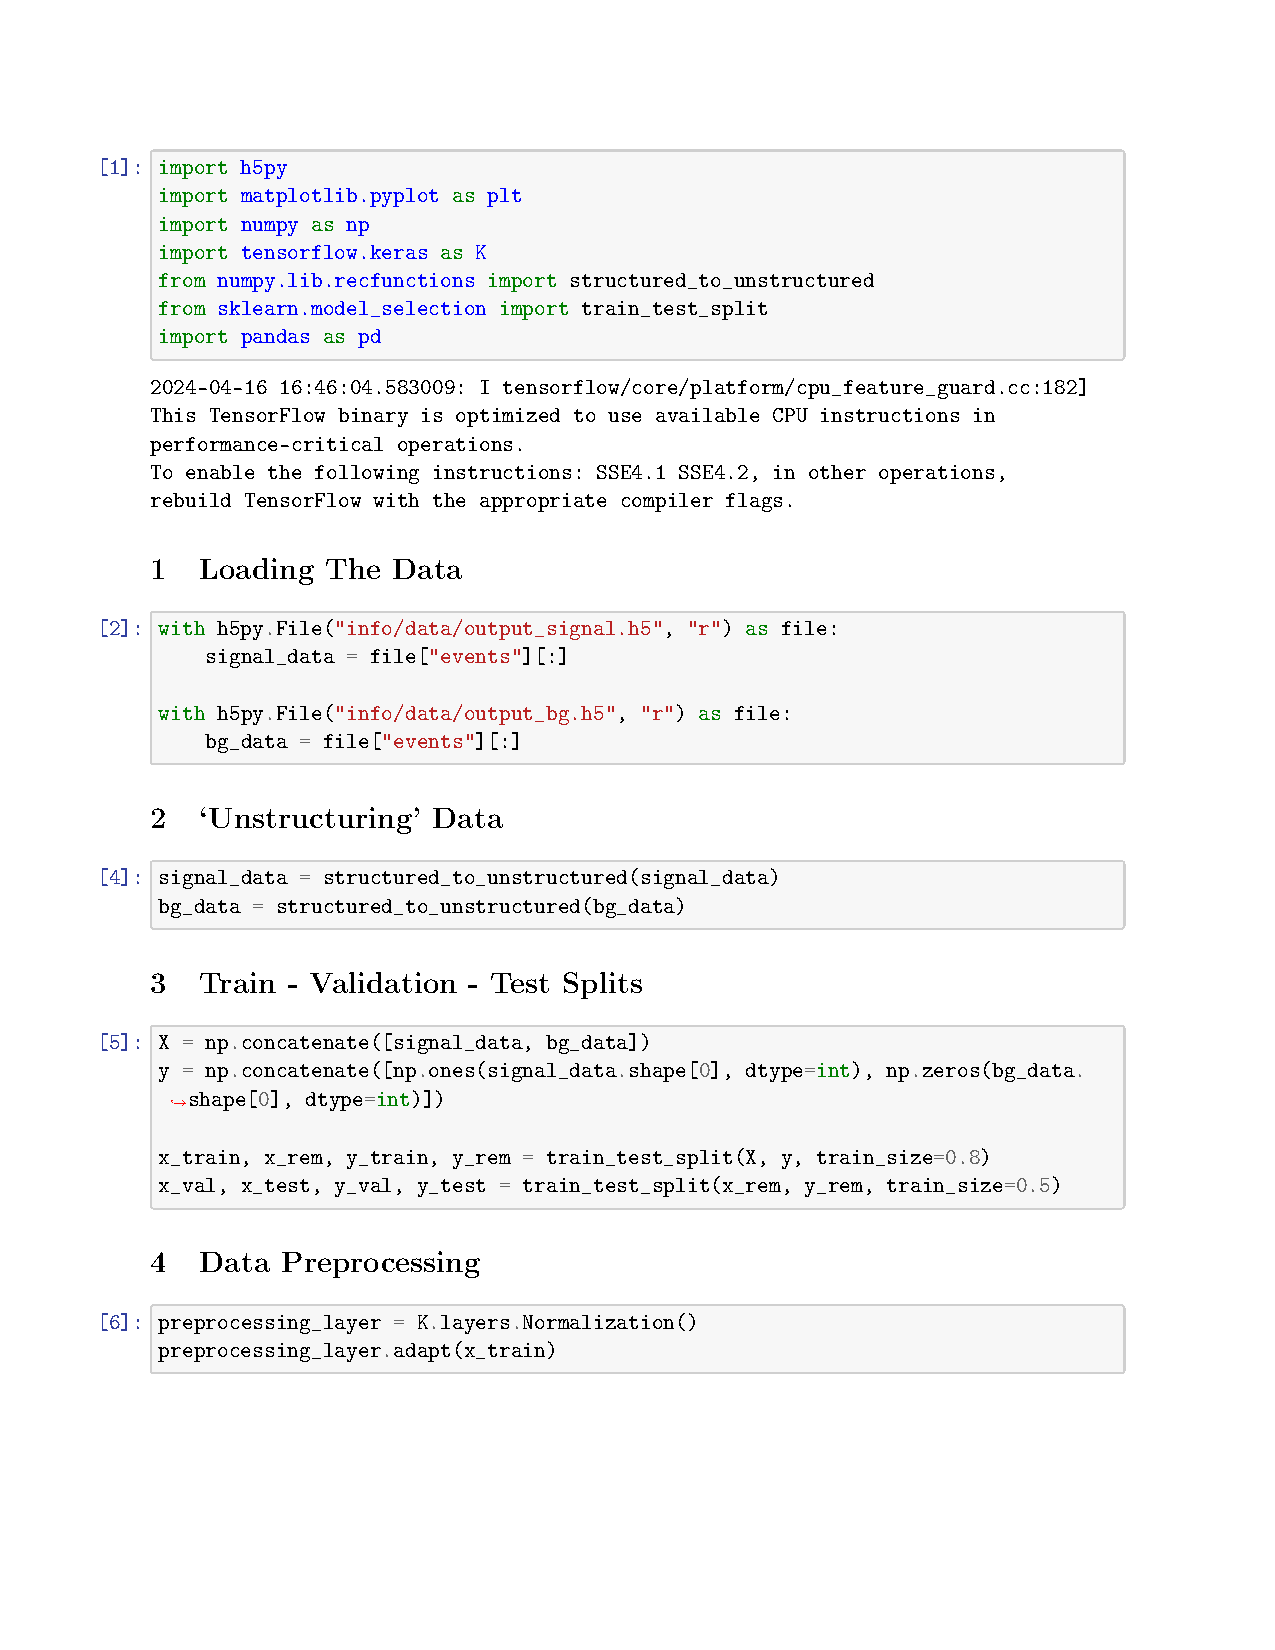
\includepdf[pages=-]{base_model/base_model.pdf}

\section{Code: Feature Selection}\label{code_feat_selection}


We present the code utilized for the Sequential Feature Selector. This code facilitated the creation of Figure \ref{fig:SFS_results} and the data compiled in Table \ref{table:SFS_results}.

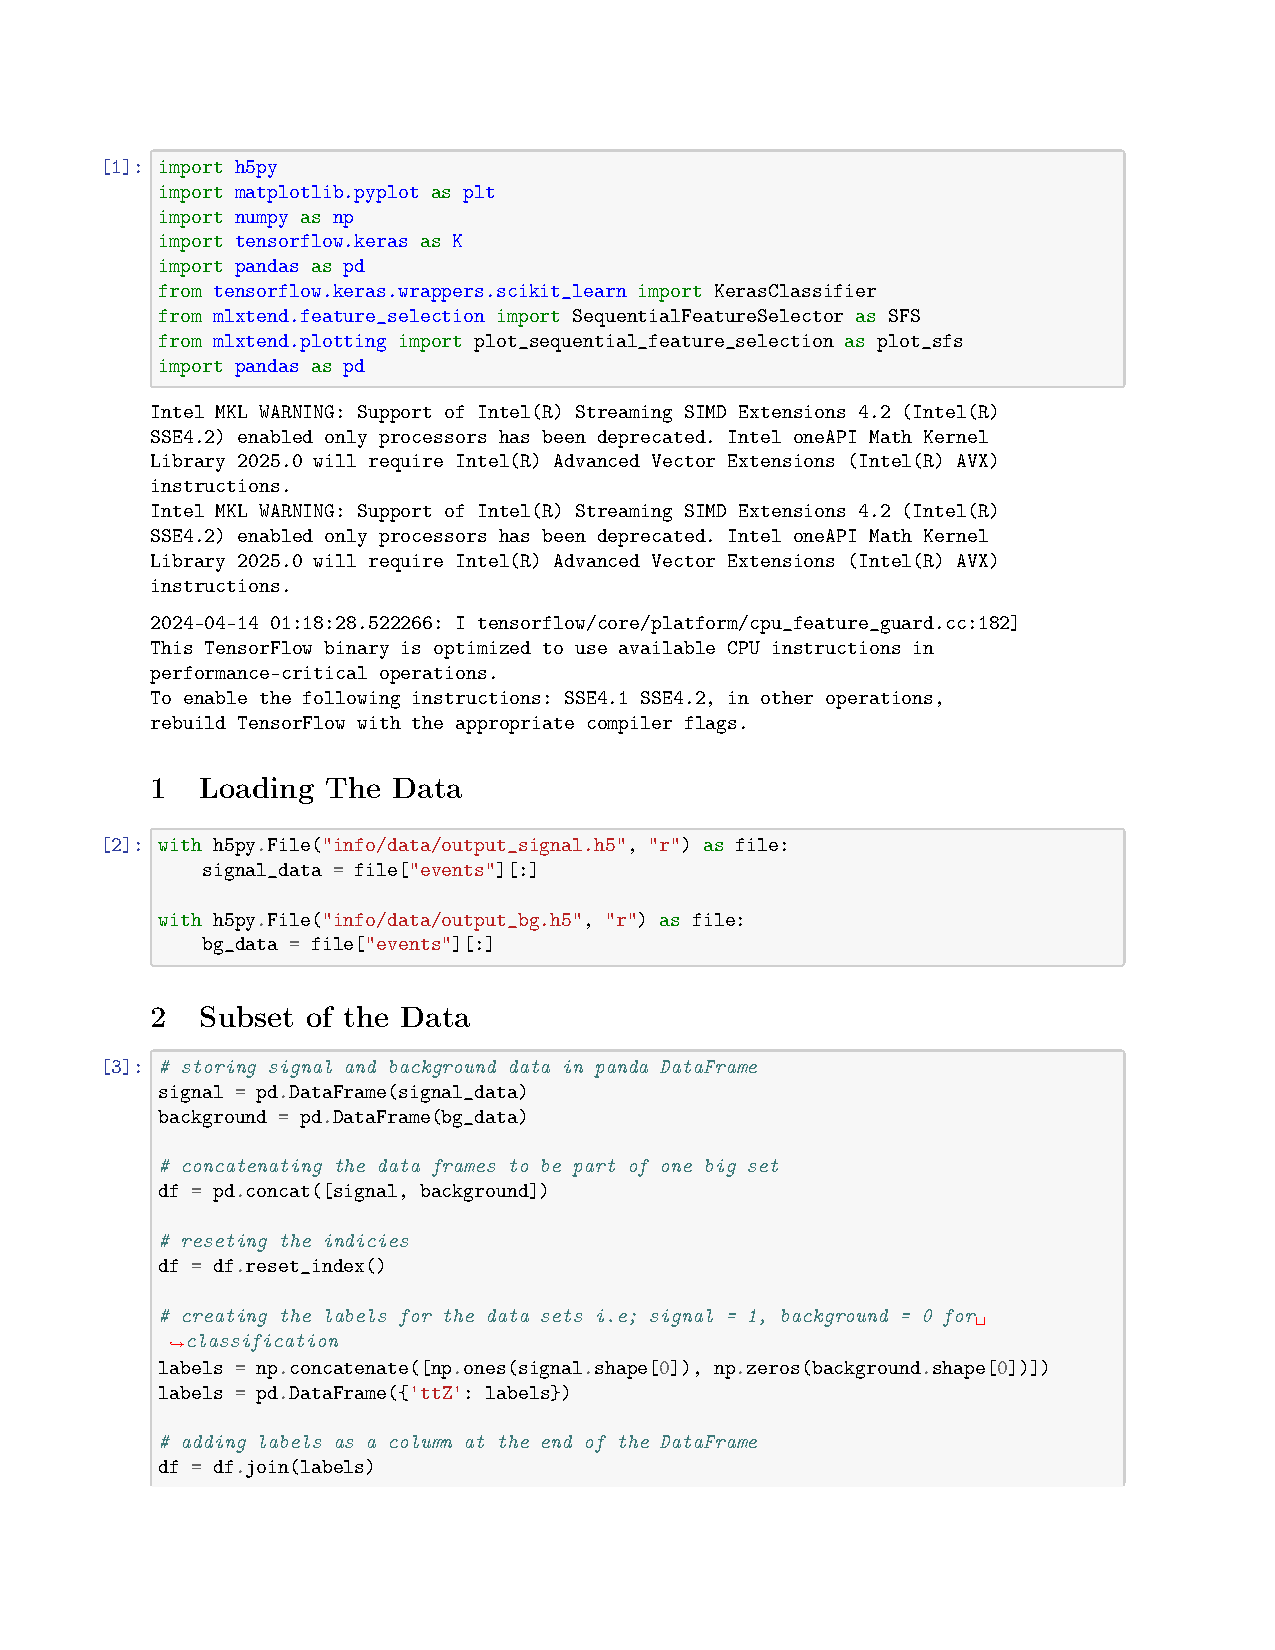
\includepdf[pages=-]{feature selection/feature_selection.pdf}

\section{Code: Feature Comparison}\label{code_feat_comparison}


We present code utilized to generate Figure \ref{fig:base_models}, which compare the performance of the base neural network model across the three feature lists.

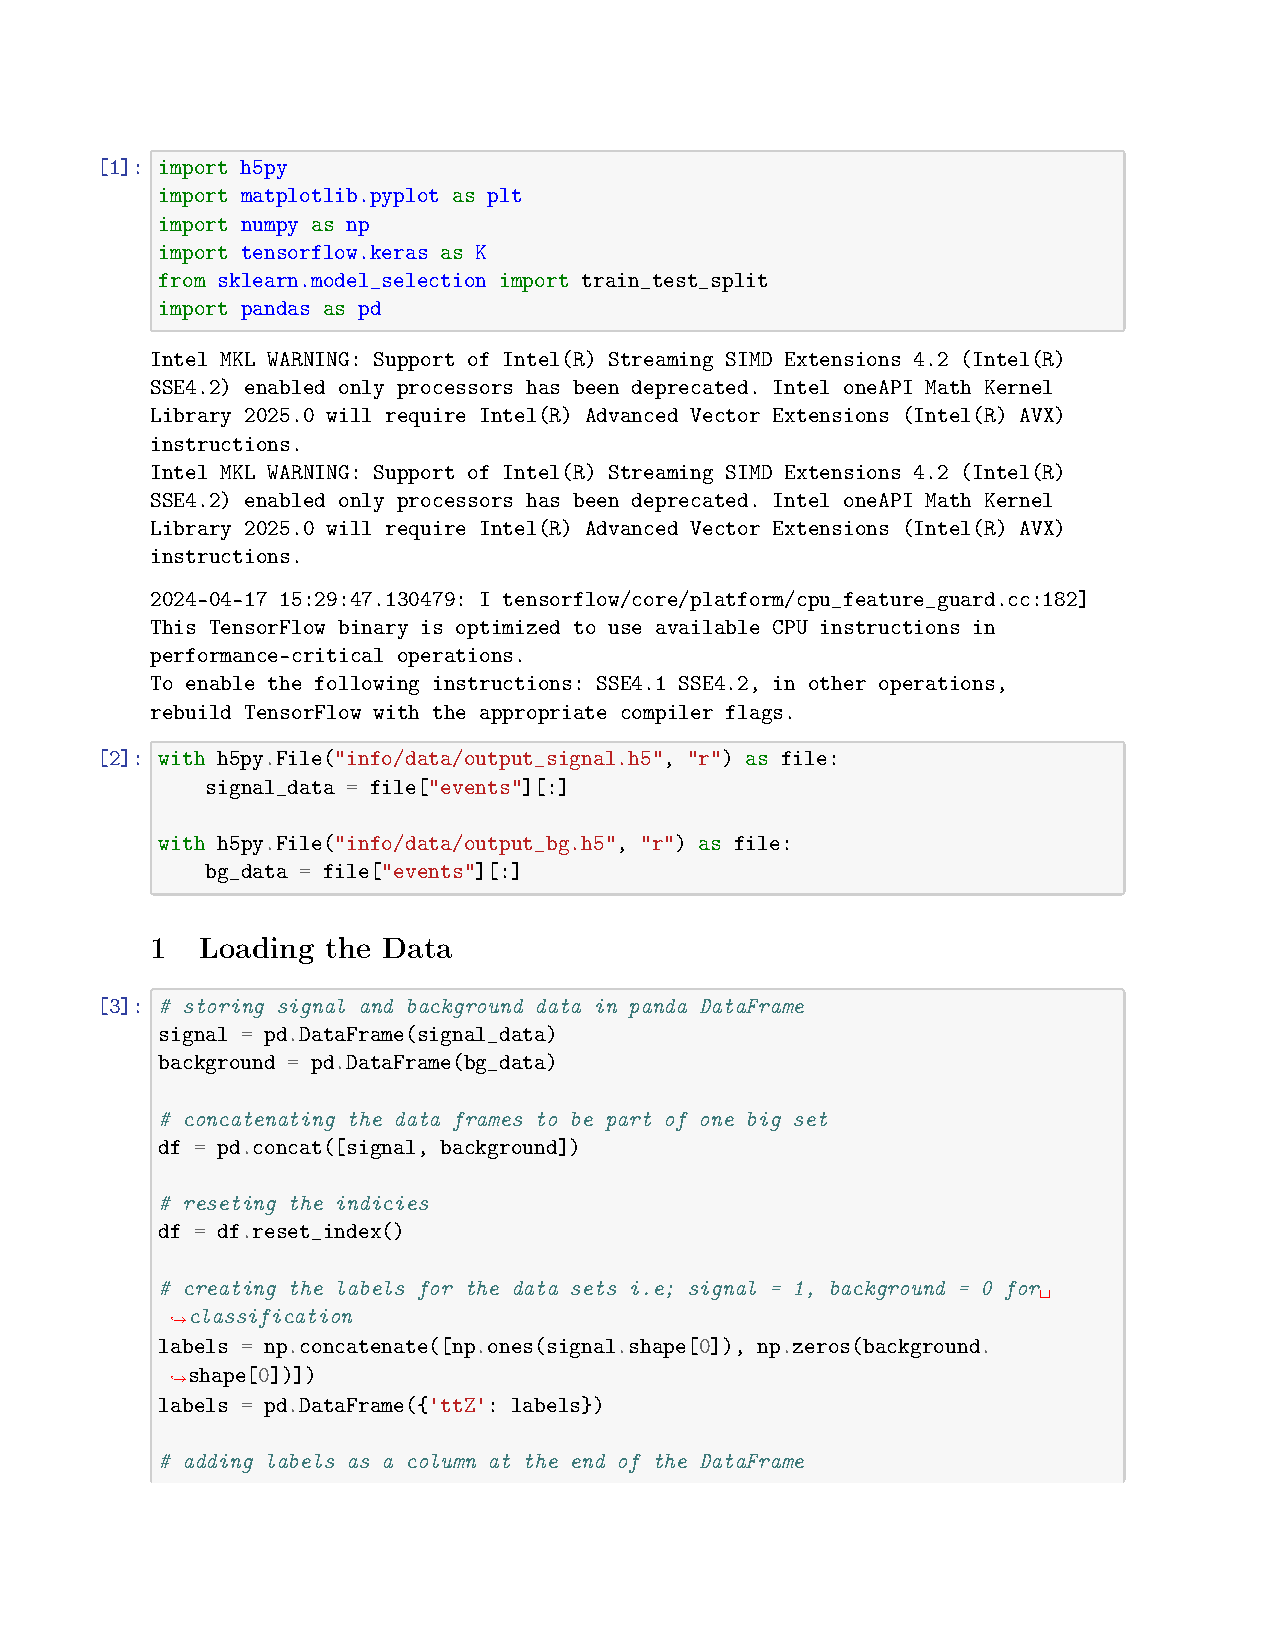
\includepdf[pages=-]{feature_comparison/feature_comparison.pdf}

\section{Code: Parameter Optimization via GridSearchCV}\label{code_model_selection}

We present code utilized for applying GridSearchCV to optimize model parameters. This code was instrumental in producing the data shown in Tables \ref{table:gridsearchCV_params} and \ref{table:best_params_gridsearchCV}.

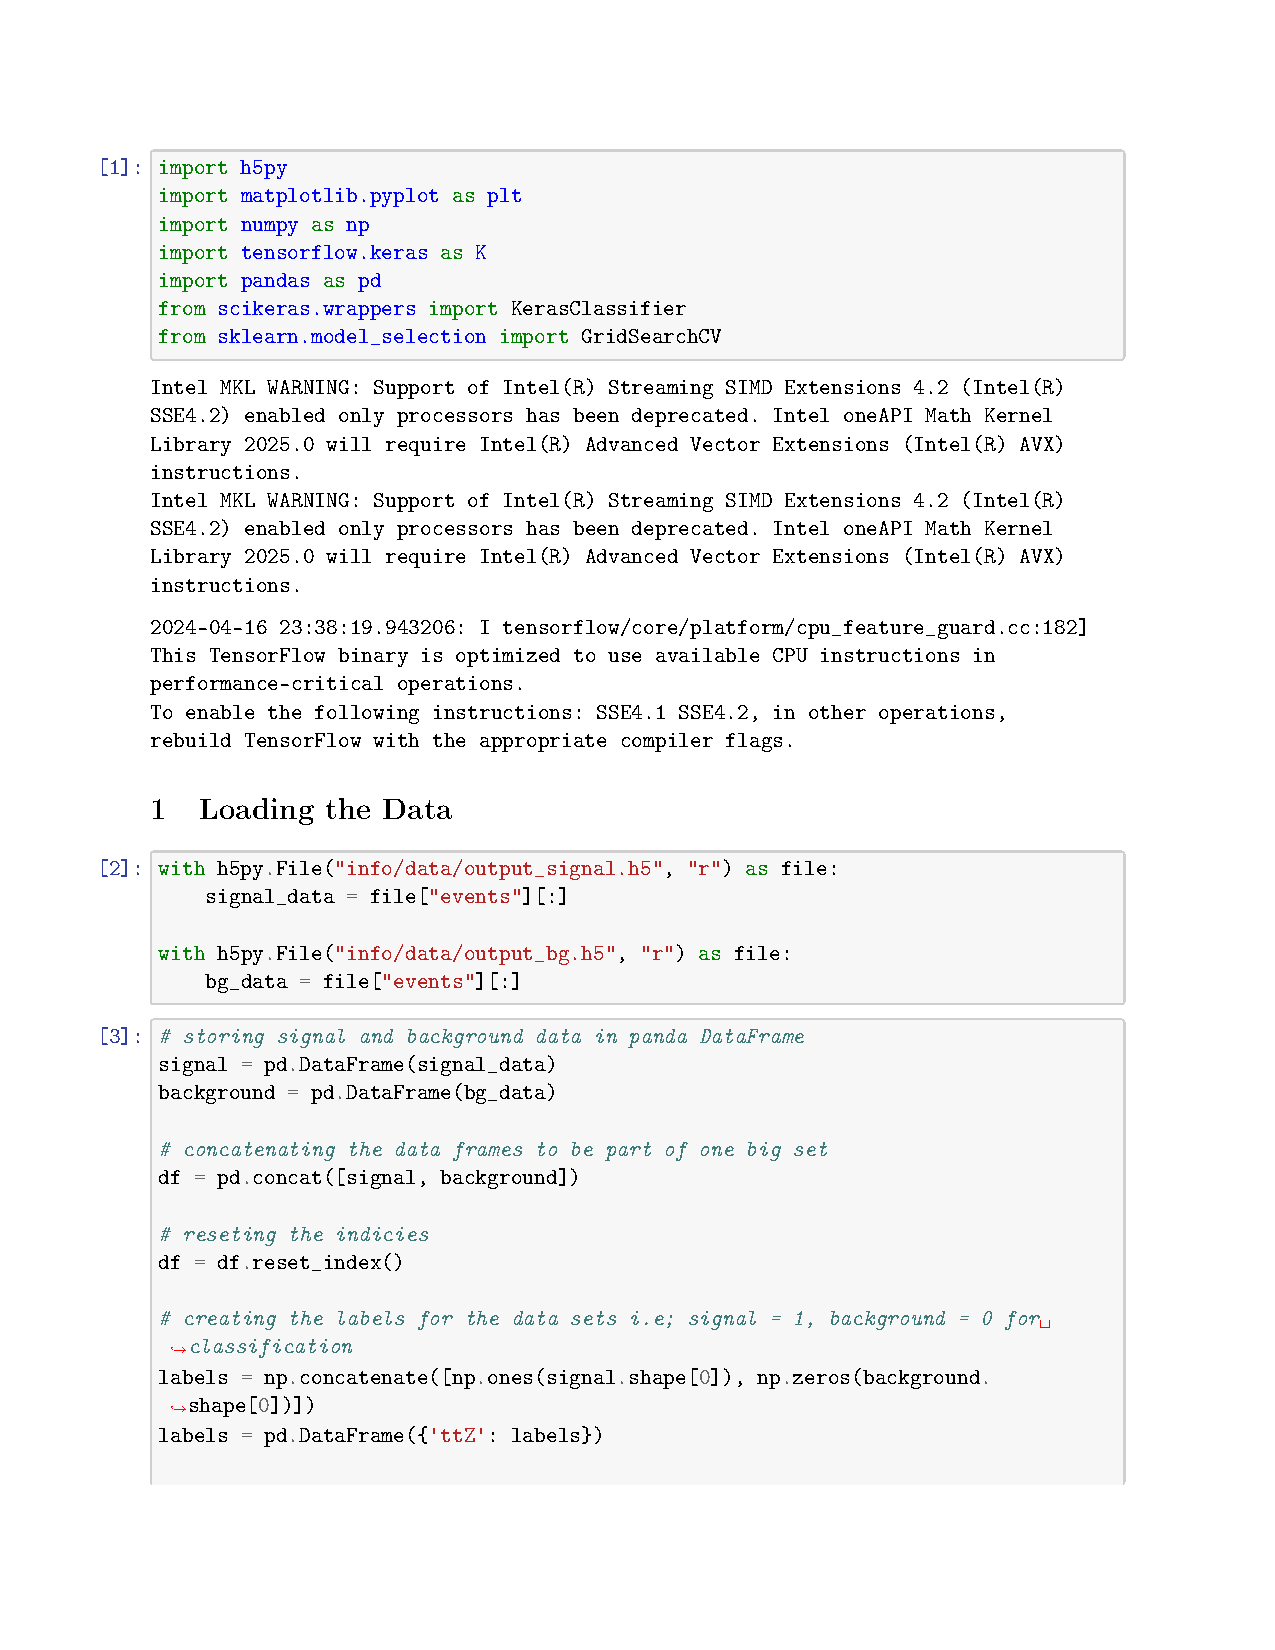
\includepdf[pages=-]{model_selection/model_selection.pdf}

\section{Code: Best Models Performance and Feature Importance}\label{code_best_models}

We present code utilized to generate the plots in Figure \ref{fig:best_models}, which compare the performance of individually optimized neural network models across the three feature lists. Additionally, this code facilitated the analysis of permutation feature importance, as displayed in Figure \ref{fig:best_models_feature_ranking}.

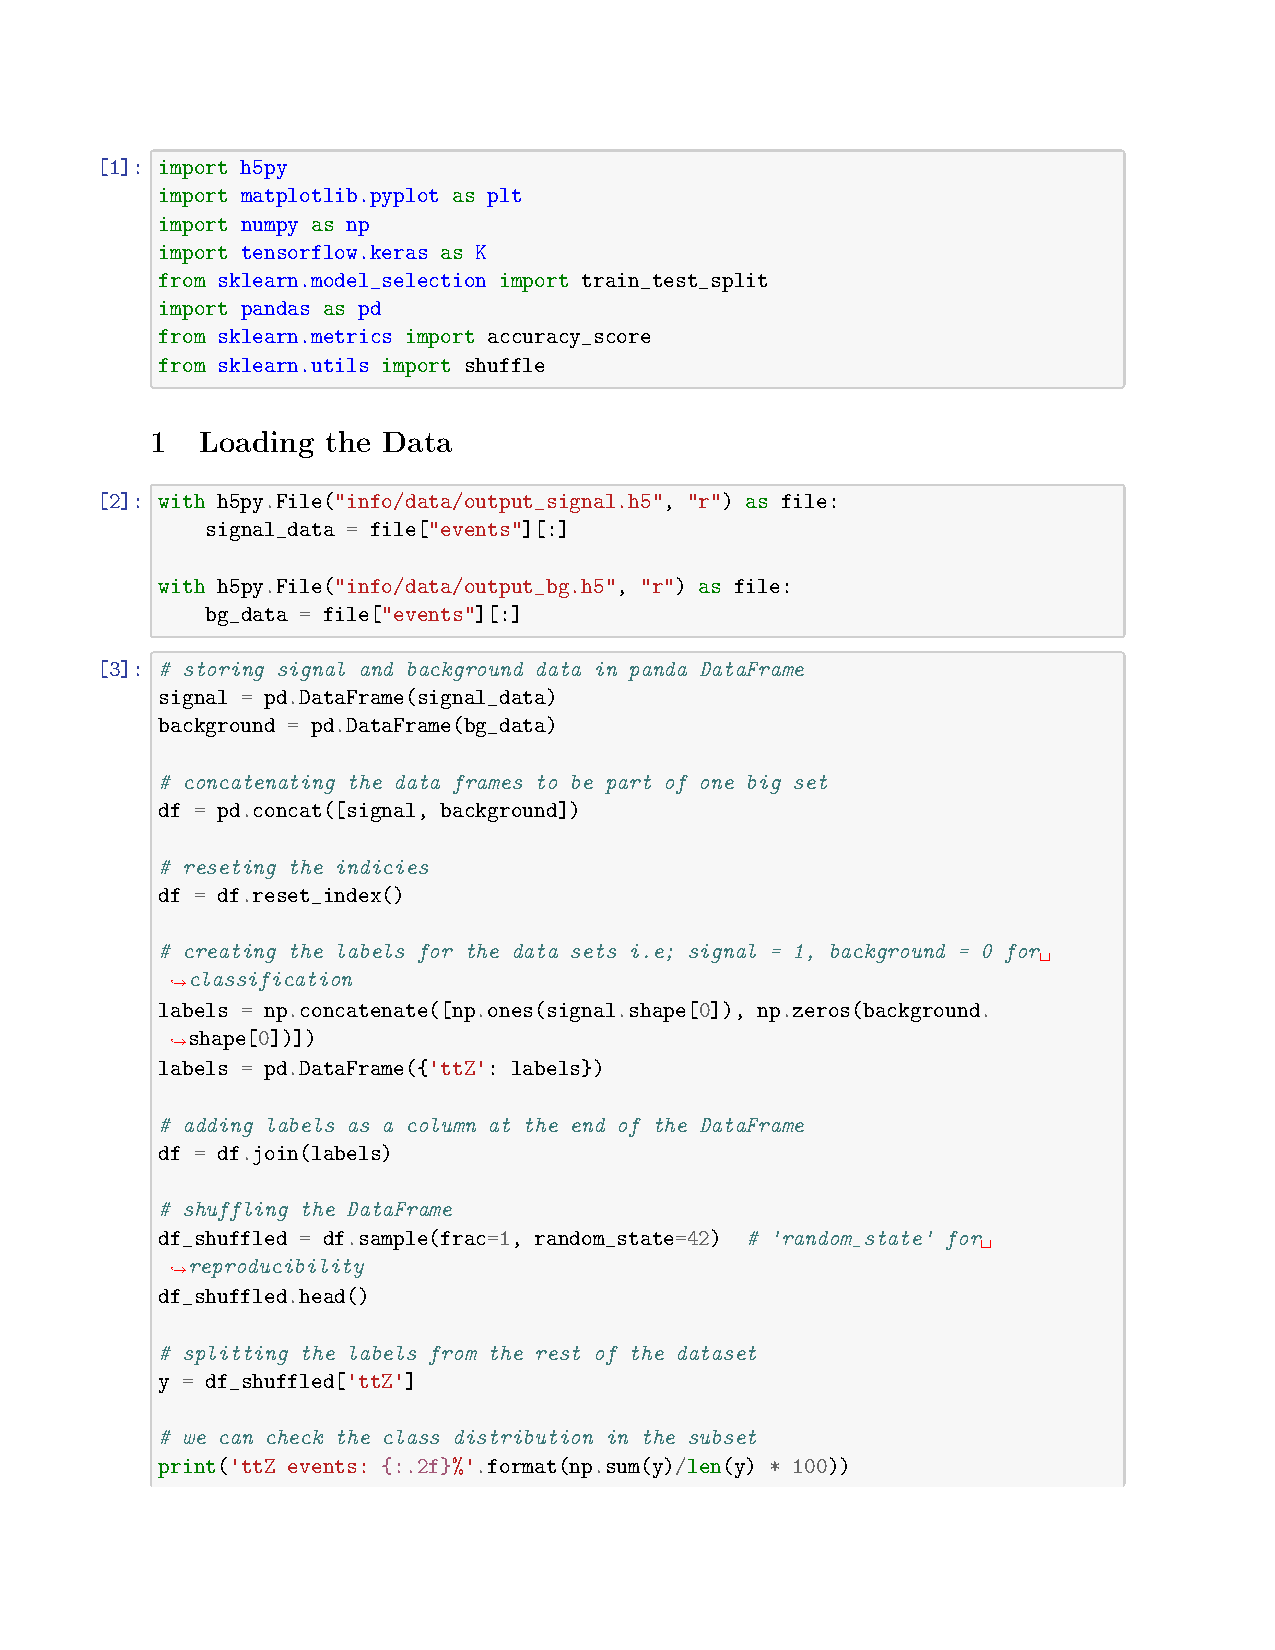
\includepdf[pages=-]{best_model/best_models_code.pdf}

\end{document}
